% !Mode:: "TeX:UTF-8" 

\BiChapter{绪论}{xu lun}
\BiSection{嵌入式智能体研究现状}{xu lun 1}
当前强化学习(Reinforcement Learning, RL)已经成为人工领域备受关注的重点之一,
它通过智能体与环境交互利用得到的奖励大小来指导策略的改进,
通过不断地试错来获得最优策略。

强化学习在游戏领域中有着广泛的应用:围棋作为经典博弈游戏,
因其具有巨大的状态空间以及复杂的策略而无法使用传统搜索算法解决,
DeepMind团队通过AlphaGo\upcite{AlphaGo}给出了基于价值函数估计和蒙特卡洛树搜索的解决方法,
首次打败人类顶级选手,标志着强化学习在处理复杂游戏中的巨大成功;
AlphaZero\upcite{AlphaZero}也使用类似模型架构,但它完全基于自我博弈学习,
在摒弃任何人类先验知识的前提下超越了AlphaGo,它展现了自博弈学习的强大能力。

类MOBA游戏(多人在线战术竞技游戏)中强化学习也有着非凡的成就,这类游戏往往有着巨大的动作、状态空间,
并带有高动态的前后文信息,需要智能体之间的团队配合能力。
OpenAI公司通过OpenAI Five\upcite{OpenAIFive}给出了基于强化学习的解决方法,
该深度网络模型为长短期记忆循环神经网络(Long Short-Term Memory,LSTM)\upcite{LSTM}和卷积神经网络(Convolutional Neural Network, CNN)组合,
提出并利用了强化学习中经典在线同策略近端策略优化算法
(Proximal Policy Optimization, PPO)算法\upcite{PPO},
使用分布式训练方法使其首次在Dota2游戏中战胜顶级职业选手。
类似的还有DeepMind团队的AlphaStar\upcite{AlphaStar}在即时战略游戏《星际争霸》中解决了复杂的多智能体决策问题。

% 在即时战略游戏(Real-Time Strategy,RTS)中,星际争霸(StarCraft)作为经典游戏,其需要玩家同时控制数百个智能体进行团队配合,
% 并需要对各类资源进行合理分配。DeepMind团队通过AlphaStar\upcite{AlphaStar}给出了基于自博弈、
% 多智能体强化学习的算法,模型采用CNN和注意力机制(Attention)处理时空信息,该模型同样超越顶级职业选手。

值得注意的是上述模型使用的算法均为\textbf{在线强化学习算法}即经典强化学习研究内容,
经典算法例如PPO\upcite{PPO}、深度Q函数学习(Deep Q Network, DQN)\upcite{DQN}、软演员评论家算法(Soft Actor-Critic, SAC)等,
这是因为\textbf{嵌入式智能体}与游戏环境之间本身具有低成本高交互次数的特性,使得智能体有无限的试错空间,可以不断对新状态空间进行探索,
更好地对动作状态价值函数$Q(s,a)$进行估计,
并进一步利用$Q(s,a)$对自身策略$\pi(a|s)$进行优化,从而通过迭代方法接近最优策略$\pi^*(a|s)$。

由于嵌入式智能体对环境信息的读取和人类完全不同,人类理解视频游戏的主要方式是通过图像信息,
而\textbf{嵌入式智能体可以直接获取精确的游戏内部信息},虽然这些人类也可以通过图像信息间接获得,
但可视化的图像信息中往往伴有噪声,在信息输入方面就会产生误差,因此就导致了游戏竞技上的不公平性产生
(其余的不公平因素,例如感知频率与操作频率,对智能加入相应限制可以解决)。

由于当前计算机视觉技术(Computer Vision, CV)发展迅速,本论文提出一种非嵌入智能体的特征提取方法,
这种\textbf{非嵌入式智能体可以仅通过获取和人类完全相同的图像信息}进行决策,
由于非嵌入式智能体只能通过模拟器和环境进行交互,无法高效获取数据,
所以本文只能收集专家数据集,采用~\ref{sec-offline-rl}~中所介绍的离线强化学习算法Decision Transformer(DT)\upcite{DT}
和StARformer\upcite{StARformer}来完成决策部分。

\BiSection{计算机视觉研究现状}{xu lun 2}
非嵌入式智能体主要利用到计算机视觉中图像分类(Image Classfication)、目标识别(Object Detection)和
光学字符识别(Optical Character Recognition, OCR)三个方面,下面分别对其进行简单介绍:
\BiSubsection{图像分类}{xu lun 3}
在图像分类任务上LeNet-5\upcite{LeNet}给出了早期卷积神经网络(Convolutional Neural Network, CNN)模型,它作为现在CNN架构的先驱之一,
在MNIST手写数据集上首次展现出深度神经网络的卓越性能。近年来由于自动微分计算速度的飞速提升以及ImageNet2012数据集\upcite{ImageNet}的支撑,
从而使得基于数据驱动的模型重新被重视,自从AlexNet\upcite{AlexNet}利用在2012年ImageNet挑战赛中取得突破性成果后,
各类新型网络架构例如VGG\upcite{VGG}、GoogleNet\upcite{GoogleNet}、ResNet\upcite{ResNet}、DenseNet\upcite{DenseNet}、
ViT\upcite{ViT}、RepVGG\upcite{RepVGG}、MetaFormer\upcite{MetaFormer}等相继被提出,这些模型不断刷新图像分类的准确率记录,同时提升了模型的计算能力和泛化能力。

研究者针对网络的宽深度(VGG)、宽度(GoogleNet)、残差连接(ResNet)、分组卷积(AlexNet)、注意力机制(ViT, MetaFormer)、模型重新参数化(RepVGG)等方面进行了深入探索,
其中残差网络的引入解决了深度网络的训练难题,可以将网络深度上升到数百层之上,乃至Transformer\upcite{transformer}类架构中也使用了残差机制;
而注意力机制的引入可以帮助模型关注图像的关键特征。
\BiSubsection{目标识别}{xu lun 4}
目标识别任务(Object Detection)旨在从图像或视频数据中识别出特征类别的目标或对象,
根据处理流程的不同检测头(Detection Head)分为单阶段检测器(Single-Stage Detectors)和多阶段检测器(Two-Stage Detectors),
其中单阶段检测器,通常为端到端问题,直接通过输入的图像给出识别框的位置(回归问题)与类别(分类问题),
当前经典模型包括YOLO(You Only Look Once)v1~$\sim$~9系列\upcite{YOLO}、
SSD(Single Shot Multibox Detector)\upcite{SSD}、DETR(DEtection TRansformer)\upcite{DETR}等。
这类算法优点在与推理速度较快,适用于实时监测任务,该系列在初次提出时检测率较低,但通过不断的优化改进,已经可以成功的解决小目标检测和重叠目标问题。
而多阶段检测器例如R-CNN\upcite{FastRCNN}系列,这类算法虽精度较高,但推理速度较长,不适用于实时监测任务。
% \begin{itemize}
%   \item 单阶段检测器(Single-Stage Detectors),通常为端到端问题,直接通过输入的图像给出识别框的位置(回归问题)与类别(分类问题),
%   当前经典模型包括YOLO(You Only Look Once)v1~$\sim$~9系列\upcite{YOLO}、
%   SSD(Single Shot Multibox Detector)\upcite{SSD}、DETR(DEtection TRansformer)\upcite{DETR}等。
%   这类算法优点在与推理速度较快,适用于实时监测任务,该系列在初次提出时检测率较低,但通过不断的优化改进,已经可以比较成功的解决小目标检测和重叠目标任务。
%   \item 多阶段检测器(Two-Stage Detectors),通常将检测过程分为两个阶段,首先生成候选区域(Region Proposals),
%   然后再对候选区域进行分类和精确定位,经典的多阶段如R-CNN\upcite{FastRCNN}系列。但这类算法由于推理速度较长,不适用于实时监测任务。
% \end{itemize}
\BiSubsection{光学字符识别}{xu lun 5} 
光学字符识别(OCR, Optical Character Recognition)目前最常用的模型是卷积循环神经网络(Convolutional Recurrent Neural Networks, CRNN)\upcite{CRNN},
其将经典序列损失问题损失函数CTC(Connectionist Temporal Classification)\upcite{CTC}与深度神经网络架构LSTM和CNN相结合,
首先利用CNN将图像信息编码为一维序列信息,再用(Bi-)LSTM\upcite{BiLSTM}进行文本预测,最后利用CTC损失函数使用对预测的文本顺序进行纠正。

但是仅有文字识别模型并不足够,还需要对图像中的文本位置进行定位再使用CRNN算法进行识别,
于是发展出了很多OCR系统,如百度公司的PP-OCRv1~$\sim$~4系列\upcite{PPOCR}。

为了理解每个模型的搭建与训练细节,本毕设对上述介绍的部分模型进行了复现\footnote{\url{https://github.com/wty-yy/katacv},复现内容包括:LeNet-5、AlexNet、VGG16、GoogleNet、ResNet50、
YOLOv1、YOLOv3、YOLOv4、YOLOv5、CTCLoss \& CRNN、miniGPT}。

\BiSection{本毕设的任务}{xu lun 6}
\begin{wrapfigure}[24]{r}{.5\textwidth} % 文字环绕行数为13行, 图片靠右 (l为靠左), 图片占0.3的行宽
  \centering\vspace*{-10ex}
  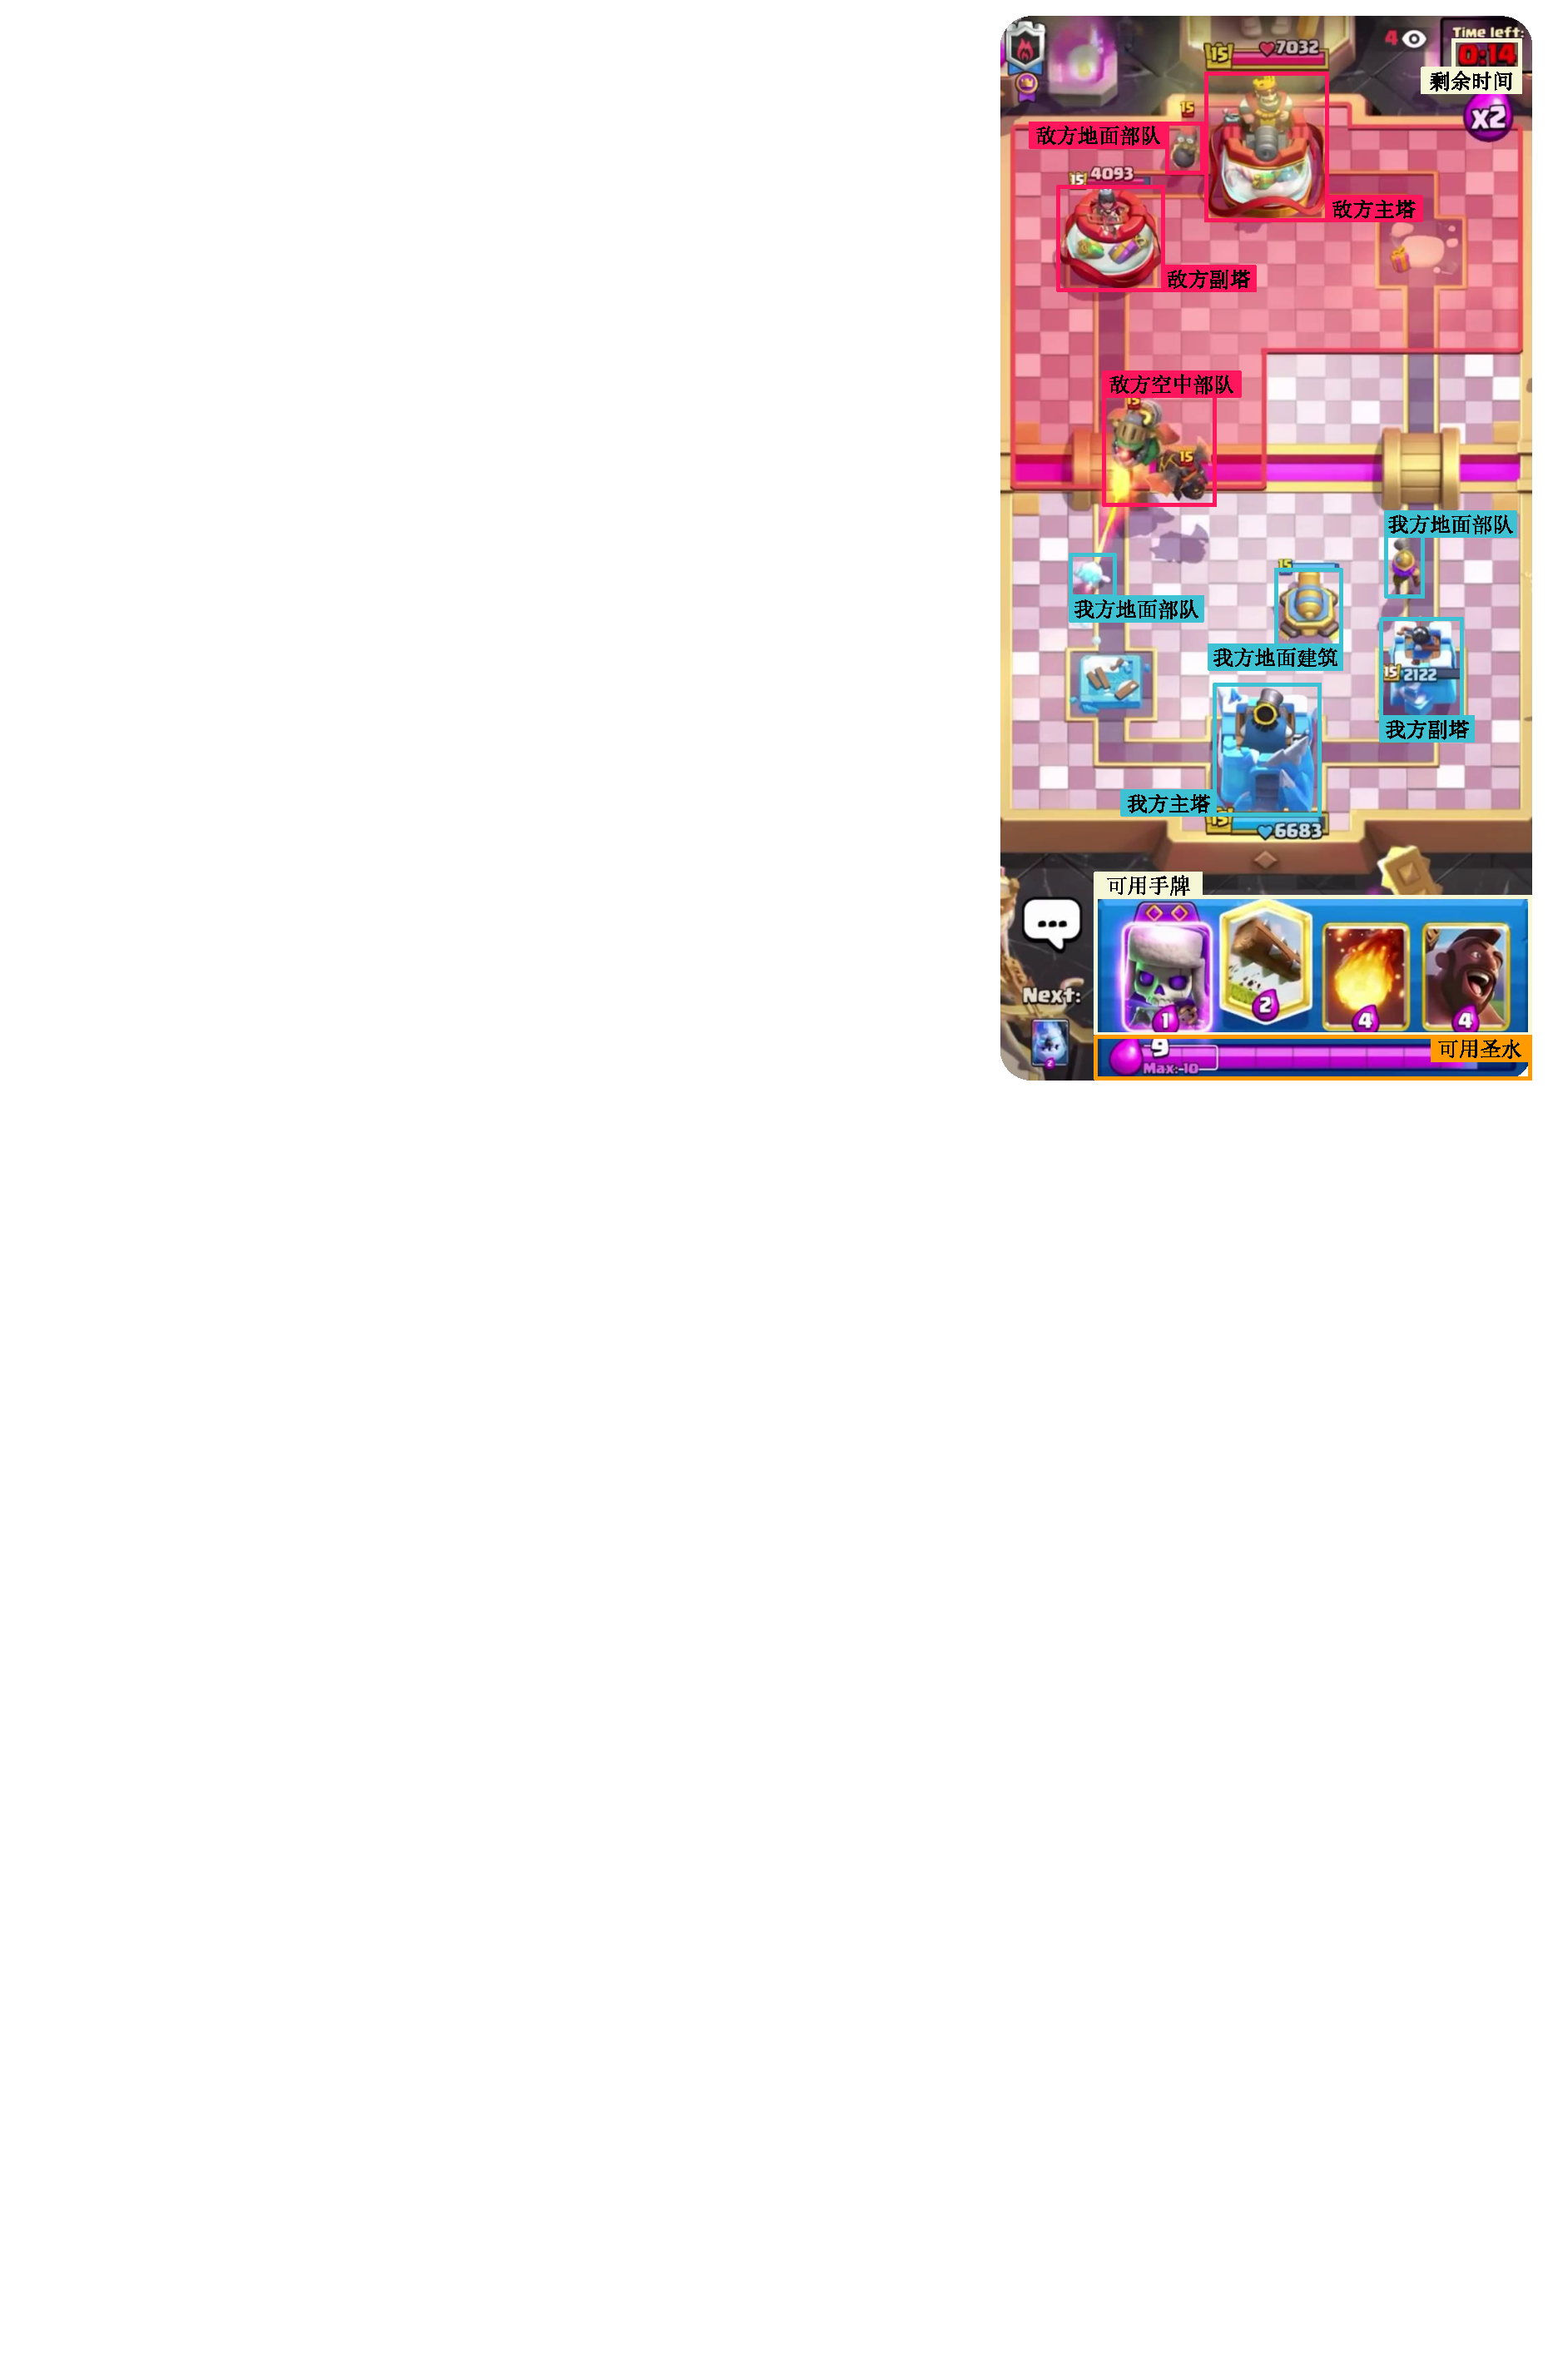
\includegraphics[width=0.5\textwidth]{introduction.pdf}
  \caption{右上角为当前阶段的剩余时间;中间部分为竞技场,其上有双方所部署的部队及建筑;
  下方显示了可用手牌以及部署所需的圣水,最下方显示了当前的可用圣水总量。}
  \label{fig-introduction}
\end{wrapfigure}
《皇室战争》(Clash Royale, CR)是一款卡牌类即时策略游戏(RTS),本文仅考虑一对一对战模式,
双方玩家需要通过实时决策使用手牌来战胜对手,首先对游戏基本规则及非嵌入式感知任务目标进行介绍:
\paragraph*{感知场景}在对局过程中,游戏场景如右图~\ref{fig-introduction}~所示,本文所需的感知内容主要分为如下四个主要部分和三个子部分:

\noindent 主要部分:
\begin{itemize}
  \item 竞技场(Arena):包括防御塔及双方所部署的部队和建筑物。
  \item 手牌:位于竞技场下方,包括当前卡片图像及其所需的圣水(Elixir)。
  \item 游戏时间:当前阶段的剩余时间。
  \item 总圣水:用于卡牌的使用,随时间自动恢复。
\end{itemize}

\noindent 子部分:
\begin{itemize}
  \item 主塔:处于三个防御塔中间,当其被摧毁时,对局直接结束。
  \item 副塔:处于左右两侧的防御塔。
  \item 部队:玩家通过卡牌部署的战斗单位,包括可移动地面和空中单位,以及建筑单位。
\end{itemize}
% 这里一定要空一行
\paragraph*{游戏目标}每位玩家的目标是摧毁尽可能多的敌方防御塔,优先摧毁敌方主塔的玩家立刻获胜。
游戏中在两种阶段下存在不同的胜利条件:\label{game-target}
\begin{enumerate}
  \item 常规时间(Regular Time):持续三分钟,目标为摧毁更多的敌方防御塔,若时间结束时防御塔数量一致,则进入加时赛,
  否则防御塔多的一方获胜。
  \item 加时赛(Over Time):持续两分钟,在该阶段中,首个摧毁敌方剩余防御塔的玩家获胜,
  若加时赛结束时仍未分出胜负,则比较双方防御塔的最低生命值,最低生命值较高者获胜,若仍未分出胜负,则为平局。
\end{enumerate}
\paragraph*{游戏过程}一次对局中每个玩家牌库大小为固定的8张,对局开始时,随机在队列中初始化卡牌的出现顺序,
每次从队首取出4张手牌,当玩家使用卡牌后,使用完的卡牌将被重新加入队尾,
所以当一方使用完8张不同卡牌时,可以通过逻辑计算出未出现卡牌类别。
玩家需要基于当前竞技场上的实时状态、手牌类别及总圣水信息,
实时决策使用卡牌的类别和位置,采取进攻或防守策略,最终按照上述“游戏目标”给出的规则判断胜负。

\BiSection{本毕设的贡献}{xu lun 7}
在本文中,首次提出一种基于非嵌入式的离线强化学习设计方案,应用于游戏《皇室战争》(Clash Royale, CR),
并最终在移动端设备上进行实时决策验证其可行性。设计方案如下:
\begin{enumerate}
  \item 生成式数据集:本文设计了一个与本任务相关的生成式数据集,使其可以模仿真实场景生成含有任意数量部队及种类的带有识别标签的图像,
  能够非常高效地生成用于目标识别的训练数据集。
  \item 感知融合:本文利用YOLOv8\upcite{YOLOv8}并结合目标追踪技术ByteTrack\upcite{ByteTrack}实现了对视频流中部队位置及类别的实时识别,
  通过PaddleOCR完成了对数字及时间信息的识别,利用ResNet完成对卡牌和圣水图标的分类,
  结合上述几种感知模型,本文还提出了一系列针对于本任务的上下文信息过滤方法用于优化感知特征。
  \item 模型决策:本文使用离线强化学习算法StARformer作为决策模型,设计相应的特征输入结构以及损失函数,
  并将难以学习的离散动作序列转化为连续动作序列进行训练,
  此方法提高了模型的决策频率与决策准确率,最后部署在手机上完成实时对局决策。
\end{enumerate}

离线强化学习模型使用手工录制的11万帧专家数据集进行训练,
能够战胜游戏内置AI,虽然无法达到$100\%$胜率,但本研究发现该离线强化学习模型能够展现出一定的模仿及泛化能力,
从一定程度上说明了这种非嵌入式离线强化学习算法的可行性。
